\documentclass[12pt]{article}
\usepackage[a4paper, total={7in, 10in}]{geometry}
\usepackage{amsmath}
\usepackage{amssymb}
\usepackage{graphicx}
\linespread{0.9}

\title{Exponents and Logarithms Lesson\vspace{-3mm}}
\author{2018-2019 SLSS Math Club\vspace{-5mm}}
\date{December 5, 2018\vspace{-5mm}}


\begin{document}
\maketitle
\section{Exponent Laws}
If $a, b, x,$ and $y$ are real numbers, the rules for exponents are:
\begin{align*}
    a^{\frac{1}{n}} &= \sqrt[n]{a} & a^0 &= 1 \text{ if } a \neq 0 & a^{-x} &= \frac{1}{a^x} \text{ if } a \neq 0 \\
    a^x a^y &= a^{x + y} & \frac{a^x}{a^y} &= a^{x - y} \text{ if } a \neq 0 & (a^x)^y &= a^{xy} \\
    a^x \cdot b^x &= (ab)^x & \frac{a^x}{b^x} &= (\frac{a}{b})^x \text{ if } b \neq 0
\end{align*}

\section{Logarithm Laws}
If $a, x,$ and $y$ are non-zero real numbers, the rules for logarithms are:
\begin{align*}
    \log_a(xy) &= \log_a{x} + \log_a{y} & \log_a{(\frac{x}{y})} &= \log_a{x} - \log_a{y} \\
    \log_a{x^y} &= y\log_a{x} & \log_a{a^x} &= a^{\log_a{x}} = x & \log_a{1} &= 0 \\
    \log_a{x} &= \frac{1}{\log_x{a}} & \frac{\log_a{x}}{\log_a{y}} &= \log_y{x}
\end{align*}

\section{Graph}
If $f(x) = a^x$ then $f^{-1}(x) = \log_ax$. The graphs of $f(x)$ and $f^{-1}(x)$ for $a = 2$ are shown below.
\begin{center}
    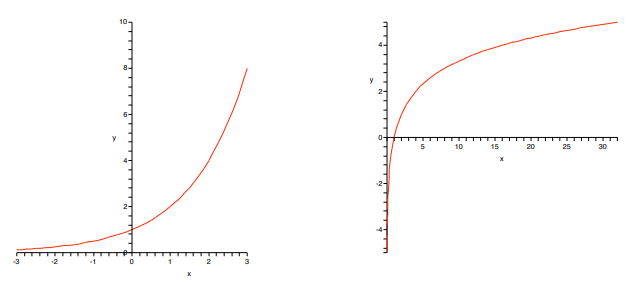
\includegraphics[scale = 1.0]{Graphics/Week_9/Graph.PNG}
\end{center}


\end{document}